\chapter{3D画像の半教師あり学習による,少量ラベルの腫瘍と正常の分類}

\section{胃がんの画像データ取得方法}

\subsection{透明化と染色}
ホルマリン固定されている検体をLUCIDによる透明化してから染色する.
多光子顕微鏡で3D画像として撮影する.一つの視野で観察することができる領域は縦横が~で深さ方向が~である.ここでLUCIDによる透明化によって今までは断面のみの撮影だったものを深さ方向まで撮影することができるようになった.
検体全ての撮影をするために画像取得にはタイリングをする.

% 三次元に撮影した画像


\subsection{擬似HE染色}

\subsection{教師データの作成}
消化器内科の医師がつけた腫瘍部分を教師データとして利用した.以下の図が腫瘍の位置をマスクした画像になっている.

\begin{figure}
	\centering
	\subfigure[]{
	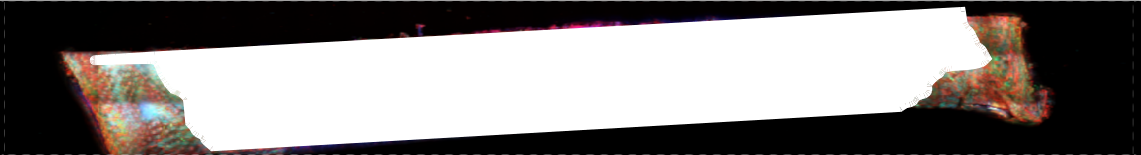
\includegraphics[clip, width=0.4\linewidth]{fig/raw_data/教師ラベル/C-010}
	}
	\subfigure[]{
	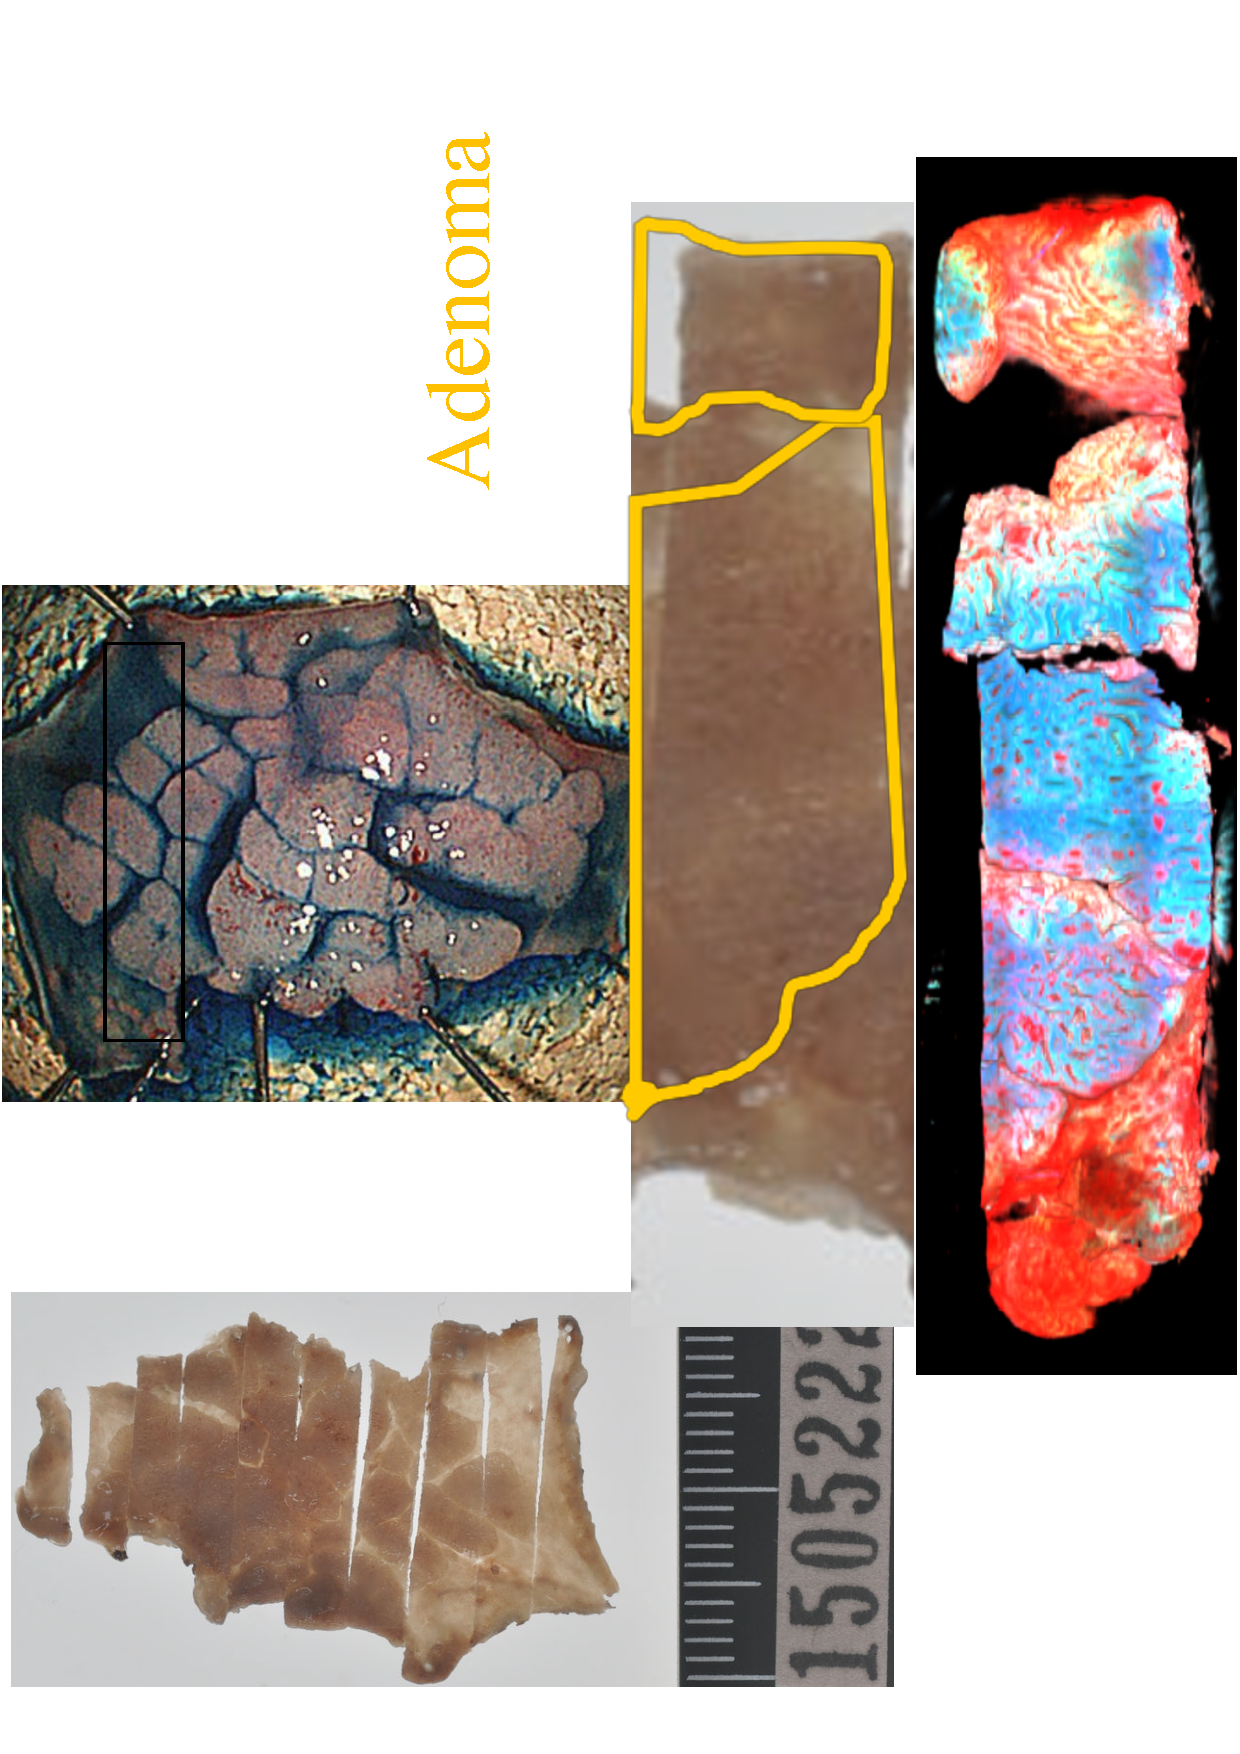
\includegraphics[clip, width=0.4\linewidth]{fig/raw_data/教師ラベル/C-011}
}
	\subfigure[]{
	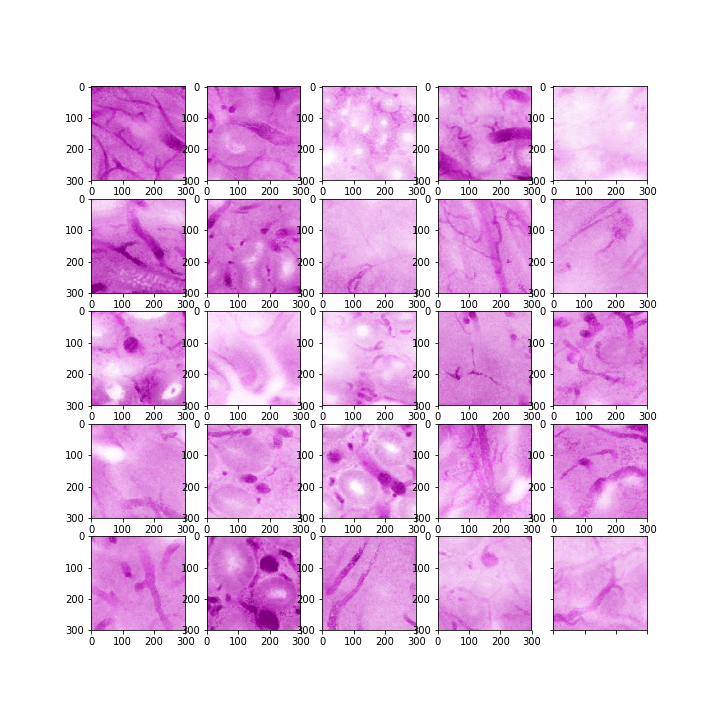
\includegraphics[clip, width=0.4\linewidth]{fig/raw_data/教師ラベル/C-012}
}
	\subfigure[]{
	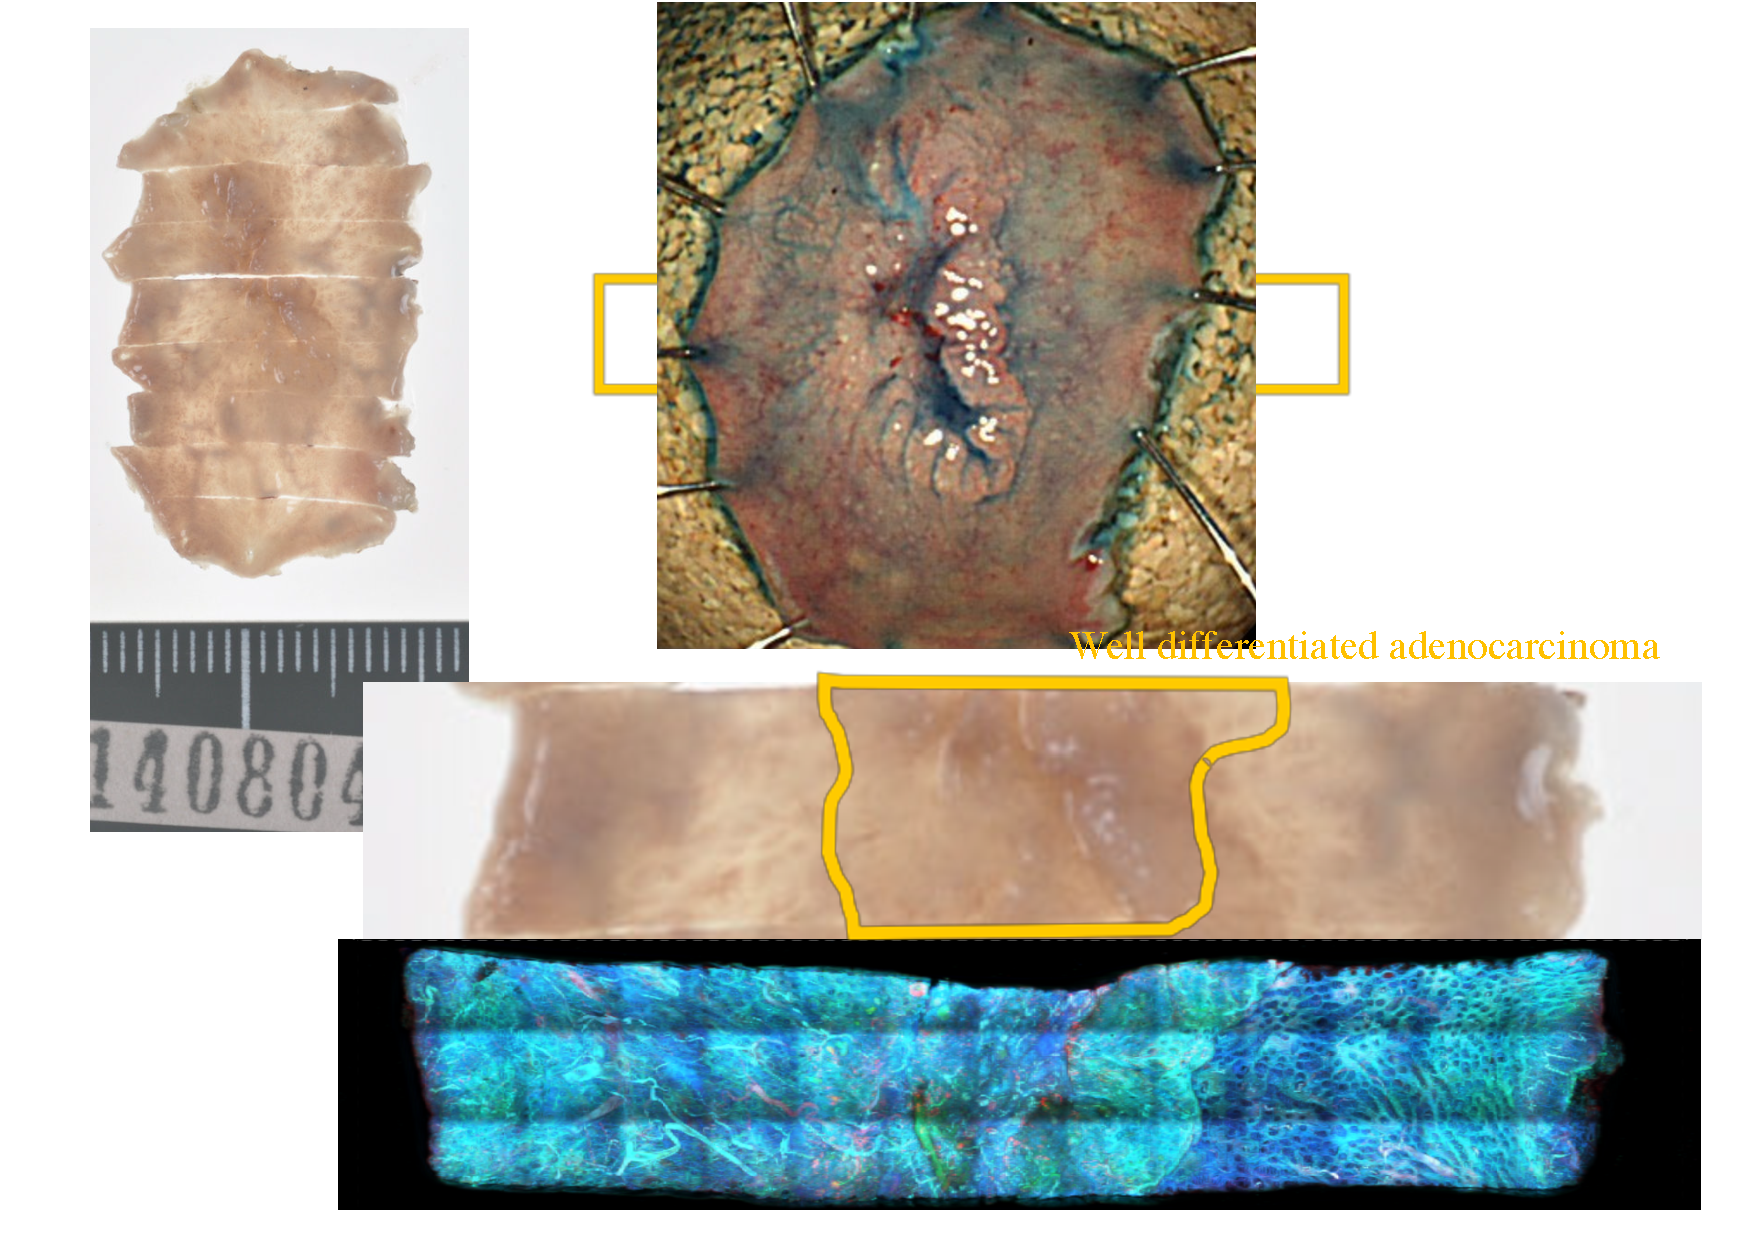
\includegraphics[clip, width=0.4\linewidth]{fig/raw_data/教師ラベル/C-013}
}
\end{figure}


\section{古典的な画像処理手法による識別精度評価}
正常と腫瘍を両方含む画像に対してHough変換による円検出で正常の線管構造を検出した.円検出では検出できない線菅構造をより多く検出するために楕円でも検出ができるように変更した.複数のパラメータを調整することで,アノテーションの正常領域が検出できるような円検出の数を増やしながらも,ノイズが多くならないような値を決定した.また,これが複数の検体で試してみた時に,最適なパラメータを見積もった.

\section{教師あり学習による識別精度評価}
\subsection*{2次元画像}
\subsection*{3次元画像}

\section{教師なし学習による識別精度評価}
\subsection*{2次元画像}
\subsection*{3次元画像}

\section{半教師あり学習による識別精度評価}
\subsection*{2次元画像}
\subsection*{3次元画像}

\section{学習環境}
Ubuntu 14.04
Github
